\chapter{Review of Institutional and Open Learning Spaces \label{cha:systudy}}
%8250
In the previous chapter it was shown that many factors need to combine to fully
support lifelong learning at universities: changes in the way of thinking of
both students and lecturers, support at the department or institutional levels,
provision of training for staff, and personal motivation of learners. This
chapter looks at \LLLs support from another angle, specifically technical
support. It reviews the area of technology and systems available for supporting
various aspects of learning, and examines how availability of a suitable virtual
learning environment may provide the \LLLs support required by students in
universities.

There are several terms that need to be clarified when discussing virtual
systems, spaces or environments. In this chapter, in order to have a common
understanding of these terms, they will have the following meaning unless
specified otherwise:

\begin{description}
	\item[Open systems:] the systems which provide users with open access and allow
	them to contribute, manage, organize, edit, use, re-use, mashup, create or
	alter content of the system \citep{Fay2009}. Such systems might even allow to
	make changes to the actual programming code of the system. Examples of the open
	systems might include Wordpress, Blogger, MediaWiki, Unix, or to some extent
	Facebook and YouTube.
	\item[Closed systems:] the systems which allow users to use content as is, with
	minimal modification to the actual system or program \citep{Fay2009}. Such
	systems are usually proprietary or have a proprietary format of content. Access
	to the closed systems is can be restricted. Examples of closed systems
	might include electronic library catalogues, online banking systems, or
	conference proceedings database.
\end{description}

The virtual learning spaces of universities are dominated by Learning Management
Systems (LMS) supporting course-related work. LMS have been started as and
still are often closed systems that require user accounts and access permissions
to the learning space. These closed systems contrast to open learning spaces
provided by Web 2.0, and social networking tools in particular, which are
characterised by open access allowing individuals to participate under their own
direction in contributing information. Social networking includes sharing,
exchanging and reflecting which provides benefits for learning. 
 
To understand the barriers and issues of utilising closed and open learning
spaces within the university environment, this chapter first explores the
currently dominant LMS and then contrasts them with the Web 2.0 virtual social
spaces. Finally, it introduces an \ep~and \ep~systems as a potential solution
that can help to close the gap that exists between the institutional and
personal learning environments. \ep~characteristics as well as the strengths and
weaknesses of selected \ep~systems are reviewed. A possible way of mapping of
the features these systems provide against the \LLLs guidelines is discussed.
This chapter concludes with an analysis investigating whether currently \ep~as a
system is mature enough to be a part of the environment that provides
comprehensive support for \LLLsn.

\section{Learning Management Systems}
Higher education institutions, universities in particular, have fully embraced
computer systems to support teaching and learning. According to a survey
conducted by the OECD Centre for Educational Research and Innovation
encompassing universities in 13 countries 89\% of responding universities were
using LMS institution-wide \citep{OECD2005}. Since then, the American Society
for Training and Development published the results of their 2009
\textit{Learning Circuits} survey according to which 91\% of their respondents
are using some kind of LMS in their organization or institution
\citep{Ellis2009}. Further indications of uptake can be seen when visiting
institutional websites, looking at user statistics provided by system suppliers
such as Moodle\footnote{\url{http://moodle.org/sites} (Accessed April 16, 2012)}
or Sakai\footnote{\url{http://sakaiproject.org/community-home} (Accessed April
16, 2012)}, or by following discussions in the academic literature \citep{Browne2006,Collis2004}.

According to Chapman \citeyearpar{Chapman2009}, there is no common definition of
a Learning Management System. A comprehensive description of LMS provided by
Watson \citeyearpar{Watson2007} states that it is a technology that can handle
all aspects of the learning process such as: delivering and managing learning
content; assessing learning of individuals and groups; tracking the progress
towards meeting learning goals; and collecting and presenting data for
controlling the learning process in institution or organization through virtual
classroom or instructor-led courses.

The systems are referred to as Virtual Learning Environments, Course Management
Systems or Learning Management Systems (LMS), the term used in this thesis. A
number of on-line information and communication tools are usually integrated in
such an environment into a single virtual location \citep{Morgan-Klein2007}. It
provides users with access to teaching and learning materials, such as lecture
slides or exercises. A virtual space within the LMS is shared by staff and
students of a particular course. This space forms a platform for course
discussions and facilitates assessment, both via on-line testing and for
submission and return of assignments.

The use of LMS in universities is characterised by a strong institutional focus
\citep{Siemens2004}. Access to the LMS depends on current enrolment with the
institution and is organised around course structures. This means students have
access to only the courses they are enrolled in or cohort based courses (e.g.
doctoral students community) and only for the duration of these courses. The
learning spaces for the different courses a student is enrolled in are separate.
LMS is based on a hierarchy of user access rights. The lecturer in charge
determines the tool-set for their course and sets the parameters that define the
involvement of the students. The lecturer has access to all information stored
for their course in the LMS, leaving no or only very limited private space for
the student. The content and use of the LMS is focused fully on the course
requirements. As a course-focused virtual learning space, LMS make a huge
contribution to the delivery of both face-to-face and distance courses in
today's universities.

Looking at all described above characteristics of the LMS, it becomes obvious
that this kind of system cannot provide required level of support for \LLLsn.
One of the reasons for this is that being managed and controlled by the
university, the LMS can only be used for formal education \citep{Venable2011}.
As a result, non-formal, informal and incidental types of learning stay outside
of institutional focus which also means that \textit{life-wide} attribute of
\LLLs is not supported. Another reason is that in the majority of the LMS,
access stops when a course finishes. This means that the LMS cannot provide
support for learning that goes outside of the time-span of the university study
and therefore cannot support \textit{life-long} attribute of learning. The last
reason lies in the \textit{self-directed} attribute of \LLLsn. As was described
earlier, LMS has a strict hierarchy of user access rights as well as control
over content, tool-set and involvement of the learners. Such conditions are
less likely to encourage users to take charge of their learning, but rather to
follow the predefined structure of their study curriculum. Due to all these
reasons, the answer to \LLLs support problem has to be sought outside of the
domain of controlled institutional environments, like LMS.

\section{Web 2.0 and Social Virtual Spaces}
Outside the higher education sector, in the open Internet domain, the Web 2.0
social networking tools have been firmly established. Tools are available for
the sharing of images, text messages, photos and video clips. Individuals can
communicate with others in synchronous and asynchronous forms, and in
access-protected as well as open formats. Individuals can consume information on
the widest possible range of topics and can as well contribute. Web 2.0 is
characterised by open access, availability to anyone who has an Internet
connection, and with the level and kind of participation determined solely by
the individual. With freedom comes responsibility, and the responsibilities for
taking up opportunities as well as for \textit{safe} conduct in the Web 2.0
space lie with the individual.

\begin{figure}[htb]
\centering
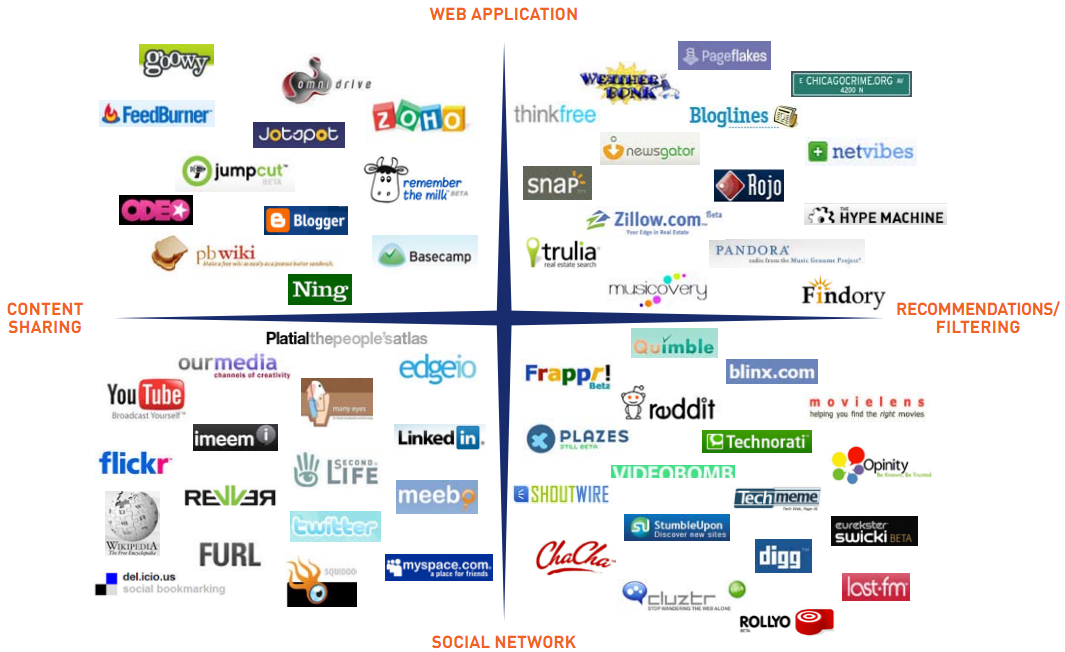
\includegraphics[width=1\textwidth]{CH4-F0-WEB20}
\caption[Web 2.0 Landscape]{Web 2.0 Landscape \citep{Dawson2007}}
%http://www.rossdawsonblog.com/Web2_Framework.pdf
\label{fig:web20l}
\end{figure}

Although there is no official classification of Web 2.0 resources, they can be
categorised as shown in Figure \ref{fig:web20l} by grouping these resources
according to their primary purpose. While this classification is not very
important for the context of this thesis, the figure illustrates the large
variety of Web 2.0 resources available online. Particularly this figure captures
only 62 Web 2.0 companies and applications considered to be prominent by
\citet{Dawson2007}. The actual number of such resources is much bigger. For
example, the largest Web 2.0 directory,
Go2Web20\footnote{\url{http://www.go2web20.net} (Accessed April 16, 2012)},
accounts for more then 3000 active resources and services, and this number grows every day showing the high
popularity of Web 2.0.

Based on statistics and publications on the Internet (as can be found by
searching for the keywords \textit{Internet statistics}, \textit{Web 2.0 statistics}, and \textit{Web 2.0
resources popularity}\footnote{As of February 2012}), the most popular Web 2.0
tools, services and resources are the ones that allow:

\begin{itemize}
  \item Create and publish information (e.g. blogs) 
  \item Collaborate with others (e.g. wikis)
  \item Network and build community (e.g. forums, social networking sites)
  \item Share personal stories with the world (e.g. podcasts)
\end{itemize}

These Web 2.0 tools promote a \textit{culture of participation}
\citep{Shelly2011} which might explain their attractiveness to the users. For
example, wikis encourage users to collaborate on creating, organizing, and
publishing information while discussing content and sharing knowledge. Whereas
wikis have become a popular tool for collaboration, blogs have been primarily
used by the individuals for various purposes. Blogs give the users an
opportunity for self-expression and sharing experience as well as promoting
their businesses or professional expertise. Another widely used way of sharing
personal stories with the world is podcasts. Such popular resources as YouTube
and iTunes allow users to upload and broadcast media files, both audio and
video. Social networking sites (e.g. Facebook, Google+, LinkedIn, MySpace) are
aimed to connect people who have common interests and goals. They give a high
level of interaction between users, a sense of community, and shared emotional
connection \citep{Zhan2010}. A notion of public opinion is present through the
commenting feature which the majority of the above mentioned Web 2.0 tools have.
In comments users can give feedback, discuss ideas, and share their view of the
topics of interest.

Web 2.0 plays an important role in today's society and is used for social and
commercial purposes. Examples from a variety of areas show the popularity and
impact of Web 2.0: virtual sports leagues attract millions of participants
\citep{Holahan2006}; politicians use blogs and podcasts in fighting for votes
\citep{Capell2006}; business models are changing, trying to adopt Web 2.0
characteristics \citep{Wirtz2010}; communication with customers is used to
increase revenue \citep{Havenstein2007}; communication pathways in research
communities are changing \citep{Ashling2007}; Web 2.0 portals are used in health
care to increase access to and enrich the quality of the information available
\citep{Gorlitz2010,Metzger2011}; video-blogging facilitates new ways of sharing
\citep{LibraryTechnologyReports2007}; the music industry is being transformed
\citep{Holahan2007}; genealogy research has become accessible to the public
\citep{MacMillan2007}; the tourism industry is adopting Web 2.0 technologies to
enhance customers' travel information and simplify access to the booking engines
\citep{Leung2011}.

Certainly, not all uses of Web 2.0 are linked to learning, especially when
thinking of the university context. But, in light of the \LLLs skills expected
from today's higher education graduates, the potential of Web 2.0 for supporting
learning becomes obvious \citep{Tian2011}. This potential is confirmed by
research studies that investigate the links between the two areas: Churchill
\citeyearpar{Churchill2009} examines the use of blogs in support of learning;
Wheeler, Yeomans and Wheeler \citeyearpar{Wheeler2008} look at student-generated
content using wikis; Boulos and Wheeler \citeyearpar{Boulos2007} investigate Web
2.0 tools for social communication in a learning context; Klamma and his team
\citeyearpar{Klamma2007} analyse a potential use of social software for
collaboration and informal learning. Yet, when designing education that
integrates Web 2.0 technologies the skill levels of students have to be
considered. While it is widely assumed that today's student generation is
Internet savvy, it has to be acknowledged that quite a number of students have
limited Web 2.0 skills. They are either not familiar with the technologies, or
have only basic level skills \citep{Kennedy2008,Hosein2010,Jones2010}.

\section{Gap Between Learning Environments}
Students in universities have access to both environments, the institutionally
controlled LMS and the participatory managed Web 2.0 resources and services. On
the whole, these two virtual worlds remain separate, both in the students' and
the institutions' minds, with a distinction being made between \textit{serious
learning} and \textit{play} \citep{Freire2008}. Many students cannot transfer
their technology skills employed in a social Web 2.0 context into academic
learning, which is both a motivational and a skill transfer issue
\citep{Katz2005}. The information technology sections of universities draw a
clear line between institutionally provided, controlled and supported LMS
services and the \textit{wild west} of the Web \citep{Havenstein2007a}. While
they cannot effectively restrict access to Web 2.0 tools, they can deny
institutional support and responsibility for quality of service. Educational
researchers and individual academics have identified the potential of social
networking tools for teaching and learning. This has led to the incorporation of
open access Web 2.0 tools into some courses at universities, as has been
illustrated earlier in this chapter.

In response to the popularity of Web 2.0 tools and their potential for learning,
LMS system providers have started to integrate social networking functionality
into their systems (as can be found in functional specifications of system
vendors). Discussion forums, blogs and wikis have been added to the tool-sets of
LMS. Yet, the important Web 2.0 characteristic of open access has been removed
as these tools have been bound into the institutional LMS framework. Access is
linked to course enrolment and under institutional control. Student-generated
content is accessible to the lecturers in charge and tool use is directed by
relevance to the respective course. The value for teaching and learning remains,
but learning is limited to the boundaries of course content and purpose
\citep{Mott2010}.

Facebook and Blackboard LMS can serve as an example that the gap between
these environments is wide and not easily bridged. An integrated application
using the Facebook social networking platform was included into the Blackboard
Learn software. Blackboard Inc. believed that such an approach would enable
students to stay connected, not only inside their classroom, but also outside
\citep{BlackboardInc.2009}. However, reviewing users' feedback on the Web (as
can be found by searching for the keywords \textit{Blackboard},
\textit{Facebook} and \textit{integration}) shows that this integration approach
was not accepted by the learner community. Users were concerned about
application security and the privacy of information stored in this social
networking environment. A number of students hesitated conducting their social
communication in such close proximity to their classroom work. 

Considerations outlined in this section bring up a need for a virtual space that
has to meet the requirements for successful \LLLs (based on Chapter
\ref{cha:litrev} recommendations) and facilitate the development of \LLLs
skills. This space has to be integrated into university environment and
accepted by student learners. It has to bridge institutional and personal
learning. The virtual space has to be safe, secure and provide students with a
long-term access. It should also facilitate both formal and informal learning
and allow for social networking and for collaboration. Such a space needs to put
students in charge of their learning and offer them privacy for exploration,
while still allowing for guidance from the lecturers. It should allow students
to continue learning informally even upon completing the formal courses (and
losing access to the LMS artifacts). This space has to provide a long-term
accessible, safe repository for storing artifacts demonstrating achievements. It
needs to be a \textit{professional} space that remains uncluttered from purely
social communication.

Taking into account all these requirements, the next section introduces \ep~as a
part of a university's learning environment that has the potential to provide
support for \LLLsn.

\section{ePortfolio}
For a long time physical portfolios have been used by artists as presentation
tools to collect, organize and showcase their artwork. The aim was to convince
potential customers of the artists' competence. Starting from two decades ago,
portfolios were adopted by educators to assess the quality of teaching
\citep{VanTartwijkJ.2004}. Since then portfolios have been used for many
different purposes and as a consequence portfolio types such as showcase,
development and assessment have been defined.
 
Electronic portfolios or ePortfolios are a digital representation of physical
portfolios. The EDUCAUSE National Learning Infrastructure Initiative
(NLII)\footnote{\url{http://www.educause.edu} (Accessed April 16, 2012)} (cited
by \citealp{IMSGlobalLearningConsortium2005}) defines ePortfolio as:

\longquote{ePortfolio is a collection of authentic and diverse evidence, drawn
from a larger archive, that represents what a person or organization has learned
over time, on which the person or organization has reflected, designed for
presentation to one or more audiences for a particular rhetorical purpose.}

\subsection{Characteristics of Portfolios and ePortfolio Systems}
\label{sec:charep}
The term portfolio is used in many different ways. As was already mentioned, an
important distinction can be made along the lines of the portfolio's purposes,
namely for development, showcase, assessment or competences
\citep{VanTartwijkJ.2004}.

Development portfolios or repositories support the learning and development of a
learner over a period of time. They contain material and artifacts related to
learning, reflections and feedback. It is important that the material stored in
these repositories is private to the learner. It is up to the learner to decide
when and what to share with whom. The learner needs to reflect on the material
collected and on his/her development in relationship to criteria or skills. The
giving and receiving of feedback are important aspects of the learning processes
around development portfolios.

Showcase portfolios tend to display examples of a learner's best work. These
presentations contain reflection and supporting evidence. They are composed for
a specific purpose and audience, e.g. a review committee, potential employer or
sponsor \citep{Lorenzo2005}.

Portfolios are often linked to assessment. The type of portfolio and type of
assessment have to be carefully adjusted to each other. Assessment portfolios
demonstrate learner's competencies and skills in well-defined areas. They can be
used for both formative and summative assessment. For formative assessment the
learner documents work and reflects on it, the assessor provides feedback that
assists the learner in future development. Summative assessment requires
predefined criteria of what is to be assessed allowing the learner to organize
work examples according to these criteria. In the design of the assessment
approach one has to be very careful to specify clearly what is to be assessed:
subject specific work, reflections, \LLLs skills, or presentation.

Portfolios for competences combine elements of both development and showcase
portfolios and are, to a certain degree, linked to assessment. In professional
areas, like health services, teacher education or engineering, the accreditation
of graduates and the continuing accreditation of professionals are often linked
to the demonstration of competencies \citep{IPENZ2007,Sullivan2004,Boyatzis2008}.
Portfolios have proven to be excellent tools for this process. The candidate
collects evidence, reflects on their practice and might invite feedback, all
processes covered by portfolio approaches. The accreditation occurs based on the
information provided in the portfolio.

Despite these variations, there are several key processes included in most if
not all portfolio work \citep{Malloff2010, Heinrich2012}, as displayed in
Figure \ref{fig:ep}.

\begin{figure}[hb]
\centering
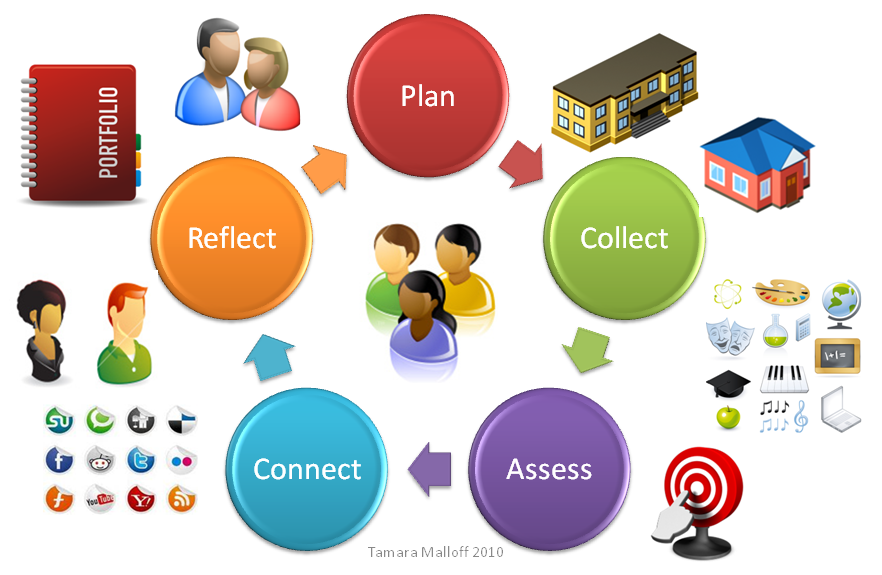
\includegraphics[height=0.47\textwidth]{CH4-F1-EP}
\caption{ePortfolio key processes}
%http://www.flickr.com/photos/kootenayleadership
\label{fig:ep}
\end{figure}

Similarly, Cambridge \citeyearpar{Cambridge2010} emphasized the importance of
the following activities in portfolio process:

\begin{itemize}
  \item Capture -- collecting/gathering information and evidence from various
  sources;
  \item Management -- aggregating captured evidence, sorting, indexing, ensuring
  accessibility over time;
  \item Reflection -- making sense of evidence, understanding own experience and
  achievements;
  \item Composition -- linking up the components together and making them
  available to others;
  \item Analysis -- understanding if additional evidence is needed, reflecting
  on feedback, keeping up dialogue with others.
\end{itemize}
 
While portfolio work can be conducted without the help of electronic systems,
such systems assist with many tasks around document collection, recording of
information, sorting through data and communicating with others. According to
Tosun and Baris's \citeyearpar{Tosun2011} research, \ep~compared to portfolio
has valuable extra features such as: a wider context and serving different
groups; archiving; cooperation and reorganization; publication and link building.
Many systems, from general Web tools to specialised applications, can be used to
support portfolio work. A comprehensive overview can be found at Helen Barrett's
ePortfolio web-site \citep{Barrett2008}. 

Using the specialized \ep~systems has its benefits over the non-specialized
approach. One of the benefits is that the specialized systems have clearly
defined centralized access control to the resources. For example, when a user
who is employing a wide range of different Web tools for \ep~work wants to share
their \ep~with others, they needs to make sure that all the artifacts in this
portfolio have the same access level and the reviewers will not come across the
``access denied'' items. In addition to centralized access control, the
specialized \ep~systems have a centralized repository which makes selecting,
aggregating and showcasing examples and artifacts easier and less time
consuming. For evaluation and feedback purposes, the specialized approach is
better for managing shared resources where the artifacts have potentially to be
locked so that changes cannot be made during the assessment time. From the
technical support perspective, the specialized systems are easier to maintain
and ensure that all users have the same high quality of services. For all these
reasons, this thesis is going to focus on systems specialised for portfolio
work.

\ep~systems are centred around the individual and their needs. They provide the
individual with a space for storing documents of any electronic format. In this
space the user creates a repository of artifacts related to all aspects of their
learning and professional development. There are tools for reflection, commonly
in form of blogs. In contrast to open Web 2.0 systems, access to both files and
reflections is by default set to the individual. Unlike in the LMS, there is no
hierarchy between users in which one higher-level user could see the work of a
lower-level user. The individual can select to share their work with others and
has full control over whom to share with and for which period of time. 

\ep~systems provide easy to use tools for constructing presentations that
combine artifacts and reflections and that can voluntarily be shared with others
or removed from public access at any time. The systems allow each individual to
form groups and identify partners for exchange. To a varying degree the
\ep~systems incorporate guidance towards reflection and self-directed learning.
\ep~systems provide a set of features that in combination are well suited to
support \LLLsn.

Each of the above mentioned features looked at separately can be found in other
computer systems or Web 2.0 tools. For example, blogs can be used for
reflection, computers' hard drives with all their disk and folder structure can
be suitable for a portfolio repository, email can serve as sharing and giving
feedback method, etc. However, the combination of these features within one
system is what makes \ep~systems so valuable.

\subsection[ePortfolio Systems Overview]{ePortfolio Systems
Overview\footnote{The \ep~systems in this section will appear in alphabetical
order.}} 
The following sections explore the features and functionality of various
\ep~systems. These specific systems were chosen for their level of success in
learning communities and current development status. Four proprietary
(PebblePad, BlackBoard \ep, Desire2Learn, eFolio) and two open-source (Mahara,
ELGG) systems are reviewed and analysed. Where possible, proprietary systems
were reviewed by accessing demonstration web sites. When demonstration web
sites were not available, the systems were reviewed by analysing user or
administrator documentation, video demonstrations, attending demonstration
seminars, and external reviews. If not specified otherwise, any material in
the systems overview can be referred back to the developer's official web site.

It is important to note here that this section is not aiming to find the best
system, but rather to evaluate \ep~systems that are currently available and
successful. Examining strengths and weaknesses of these systems can provide a
better foundation for understanding and development of an \ep~aided environment
that can provide comprehensive support for \LLLsn.

\subsubsection{BlackBoard ePortfolio}
In 2006, a popular LMS provider
BlackBoard\footnote{\url{http://www.blackboard.com} (Accessed April 16, 2012)}
developed an \ep~toolkit the most recent release of which is currently a part of BlackBoard Learn 9.1.
This \ep~system is designed as an add-on to the LMS environment and cannot be
used as a stand-alone product. On one hand, it means that all users must have
BlackBoard LMS account to be able to access \ep. On the other hand, it gives
some advantages which other \ep~systems might lack, such as single sign-on with
LMS, direct import of graded materials from Blackboard courses and links to
course goals and objectives.

BlackBoard \ep~is available in Basic and Personal Portfolio versions. Basic
Portfolio has an \ep~set-up wizard for learners who need guidance. However, it
is largely dependent on functionality available in the LMS. Without activation
of various features, the repository might be restricted to text and hyper-links
only. Personal Portfolio provides more flexibility and functionality. Therefore,
this version will be reviewed further as BlackBoard \ep~(Figure \ref{fig:bbep}).

\begin{figure}[htb]
\centering 
\setlength\fboxsep{0pt}
\setlength\fboxrule{0.5pt}
\fbox{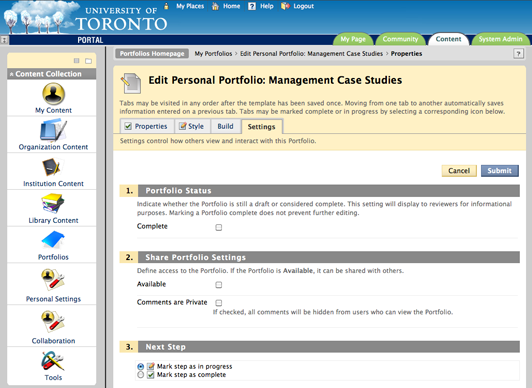
\includegraphics[width=0.9\textwidth]{CH4-F6-BB}}
\caption[BlackBoard ePortfolio example]{BlackBoard ePortfolio example
\citep{UniversityofTorontoScarborough2010}}
\label{fig:bbep}
\end{figure}

In the system, ePortfolio owners have control over the content, access, layout
and style of their portfolio. ePortfolios can be created from available
templates predefined by an administrator or a lecturer, or they can be created
from scratch. A variety of video, audio and text file types is supported as well
as an HTML editor for creating pages. Reflections are facilitated in the form of
blogs or threaded topics. Content is separated from portfolios which allows
reuse of the artifacts. It has been reported that because of this separation
artifact management is not intuitive and might be too complex for students for
effective use of the tools \citep{Clark2009}. In addition, portfolios can be
linked to learning objectives defined by lecturers, administrators or learners
themselves.

When necessary, BlackBoard \ep~can be shared with people inside the
institutional community through system username, groups and courses as well as
outside -- via email or creating a guest account which is by default active for
30 days. However, availability of these sharing options is set up by system
administrator who can allow or restrict any of these options. Depending on
access level, users can leave their feedback in the form of comments. Comments
cannot be attached to individual artifacts and are stored within single pages of
\ep. BlackBoard \ep~system has a basic reporting system where users can enable
tracking, and gather basic data about views of their portfolios. At the
completion of studies \ep~can be downloaded and saved as HTML in a ZIP archive.

Overall, BlackBoard \ep~is good for creating portfolio of student course or
program work and for linking to a course of study
\citep{UniversityofTorontoScarborough2010}. 

According to \citet{Sweat-Guy2007}, the cost of 12 months license for
BlackBoard \ep~in 2006-2007 was 20,900USD per institution which did not include
the cost of prior purchase and adoption of LMS. To date, no information was
found on current development status and future releases.

\subsubsection{Desire2Learn}
Desire2Learn\footnote{\url{http://www.desire2learn.com} (Accessed April 16,
2012)} \ep~is a proprietary \ep~system developed by Desire2Learn Incorporated. It can be deployed as a
standalone application or as a part of a Desire2Learn Learning Environment. As a
result of close working relationship of the developing company with Microsoft,
this \ep~system, as well as all Desire2Learn software, is built on Microsoft
technologies, such as SQL Server and Windows Server \citep{AAEEBL2011a}.

Most artifacts can be uploaded to the system from external resources. Some of
them, such as HTML files, can be created within the environment. This also
includes creating audio recordings which is a unique functionality compared to
other \ep~systems. Currently, Desire2Learn developers are looking into adding
support for creating of video records.

There is a standard range of functionalities associated with artifacts in this
ePortfolio system: they can be grouped, shared with others, commented on,
assessed directly or submitted as an assignment. Assessment results, such as
grades, competencies or quiz details, can be saved as \ep~artifacts as well.

\begin{figure}[htb]
\centering
\setlength\fboxsep{0pt}
\setlength\fboxrule{0.5pt}
\fbox{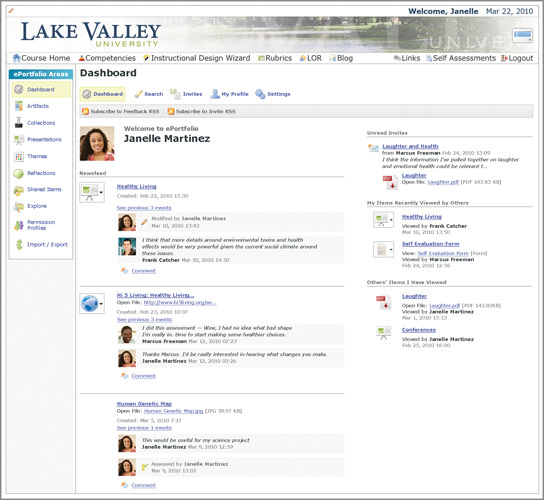
\includegraphics[width=0.9\textwidth]{CH4-F7-D2L}}
\caption[Desire2Learn ePortfolio example]{Desire2Learn ePortfolio example
\citep{Desire2LearnIncorporated2011}}
\label{fig:d2ep} 
\end{figure}

In addition to individual artifacts, other types of items in the \ep~system are
collections, presentations, reflections and forms. Collections are used to group
artifacts and can be created manually or automatically based on a defined tag
set. Forms provide a way of developing artifacts with standard field types. This
can be used for creating templates for evaluations, resumes, or self-evaluation.
Presentations are personal web sites that present a set of artifacts in an
organized way allowing users to choose theme, set up layout and manage content
(Figure \ref{fig:d2ep}). Reflections are a separate form of the artifacts. They
can be associated with artifacts or presentations and can be a part of
collection or presentation.

Feedback can be applied to individual artifacts, collections, reflections or
entire presentations. If needed, evaluators can review all comments made by
peers. Users can add assessment rubrics to artifacts that require specific
type of evaluation. More comprehensive assessment features are available via
integration with other Desire2Learn LMS tools. 

Desire2Learn \ep~has reporting capabilities for administrators and teachers
which support tracking usage and accessing detailed information on competency
achievement by students. Minor reporting is available to users in form of
presentations access logs.

Any part or an entire \ep~contents can be imported or exported using either XML,
or HTML format. XML is a native format of the system and allows the import of
\ep~to another Desire2Learn \ep~system instance.

No estimate cost of the Desire2Learn \ep~was discovered as vendors do not
disclose pricing information, explaining that each case is unique to each
institution.
 
\subsubsection{eFolio}

The eFolio\footnote{\url{http://www.avenetefolio.com} (Accessed April 16, 2012)}
system is a software service hosted and maintained by Avenet Web Solutions. Developed in 2001
together with the University of Minnesota, eFolio currently has a large user
base, the biggest of which are
eFolioMinnesota\footnote{\url{http://www.efoliominnesota.com} (Accessed April
16, 2012)} (over 60,000 active users) and
eFolioWorld\footnote{\url{http://www.efolioworld.com} (Accessed April 16, 2012)} (over 34,000 active users) \citep{AAEEBL2011}. Although eFolio is a hosted service, it
is still possible to get self-hosted solutions for very large implementations.

Every account in eFolio can have multiple portfolios which are organized as
sites. When users start creating a site, they can use a wizard under the ``To
Do" category for filling the pages with the relevant content. The latest version
of the system has a drag and drop site management interface which makes it easy to
create sites and pages. eFolio comes with a number of build-in display and style
formats. However, according to the comments \citep{AAEEBL2011}, the system
does not provide as much page layout flexibility as some users would expect.

Everything saved in eFolio is located in the ``My Content'' category. Currently,
its standard storage capacity is 50MB per user, but this limit can be
negotiated. My Content groups items by data types such as artifacts, courses
taken, goals, images, URLs, employment, etc. As well, users can add or create
the items on the fly while building their sites. Users can set up content
properties and formatting, add other content related to the item and write
multiple reflections.

All sites are by default private, but can be set to public once finished.
Under-age user sites are always private by default and cannot be made public.
Alternatively, owners can invite a specific person to review their site. Access
to the web site is granted through creating visitors. Each visitor gets an email
with login details if the site is private or site URL if it is public. Even
users who already have accounts in the system get a visitor account for each
specific site access. Visitors can leave feedback to any item with feedback
properties set up. Depending on these properties, feedback can be in the form of
Likert scale, question/answer or free-form text.

\begin{figure}[htb]
\centering
\setlength\fboxsep{0pt}
\setlength\fboxrule{0.5pt}
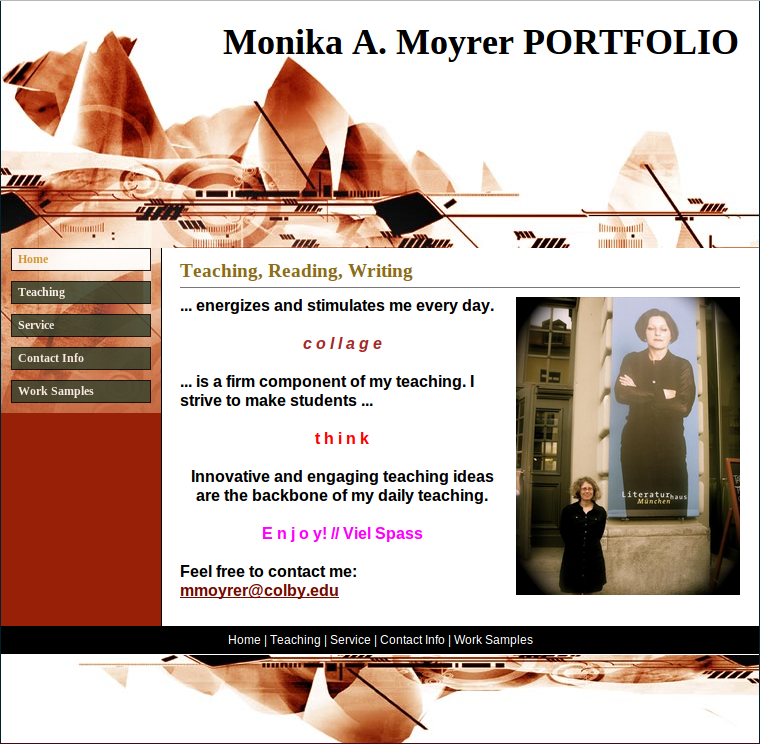
\includegraphics[width=0.87\textwidth]{CH4-F8-eFolio}
\caption[eFolio system example]{eFolio system example \citep{EFolioMinnesota2011}}
\label{fig:efolio}
\end{figure}

eFolio does not provide collaboration functionality and all web sites in the
system are personal (Figure \ref{fig:efolio}). For assessment purposes eFolio
has questionnaires of various types which students can use to address assessment
criteria.

eFolio supports the IMS ePortfolio standard \citep{AAEEBL2011} which allows
users to import/export their ePortfolio content. The system can be integrated
with the Moodle LMS. However, no detailed information was found on what kind of
integration this is.

After graduating or leaving a sponsoring institution, users can continue
using their eFolio for an annual fee of 15USD. Prices for institutions depend
on numbers of users, and can range between 15USD - 4USD per user
\citep{AAEEBL2011}.

\subsubsection{ELGG}
ELGG\footnote{\url{http://elgg.org} (Accessed April 16, 2012)} is an open source
social networking and social publishing platform started in 2004 and released under the GNU
General Public License
v2\footnote{\url{http://www.gnu.org/licenses/gpl-2.0.html} (Accessed April 16,
2012)}. It was originally aimed at higher education, but is currently used in many contexts from business
to sport. Developers of ELGG call it a \textit{social engine to empower social
environment}.

Features available in the standard platform installation include user management
and administration, social networking components (like friends list and ``the
wire''), blogging, message board, file repository, private messaging, pages, and
bookmarks. Additional components can be installed by administrator as plugins
and can be used within the entire system.

Most the end-user functionality comes from plugins which can be loaded into the
system. This review examines a standard installation. ELGG is supported by an
extensive community which has contributed a large number of plugins. In general,
most of these plugins are aimed at supporting social networking.

Unlike other ePortfolio systems, ELGG has a quite limited choice of permissions.
Artifacts in the system can be either private/public, or shared with friends
or logged-in users. There is no way of having multiple permission settings or
user-to-user permissions for artifacts.

In ELGG, each account has a profile page (Figure \ref{fig:elgg}) which links to
all available artifacts created by the user through adding or removing widgets.
Except for the profile page, there is no standard way of aggregating artifacts
for presentation. The profile page is as well the main option for showcasing as
users cannot have multiple ePortfolios.

\begin{figure}[htb]
\centering
\setlength\fboxsep{0pt}
\setlength\fboxrule{0.5pt}
\fbox{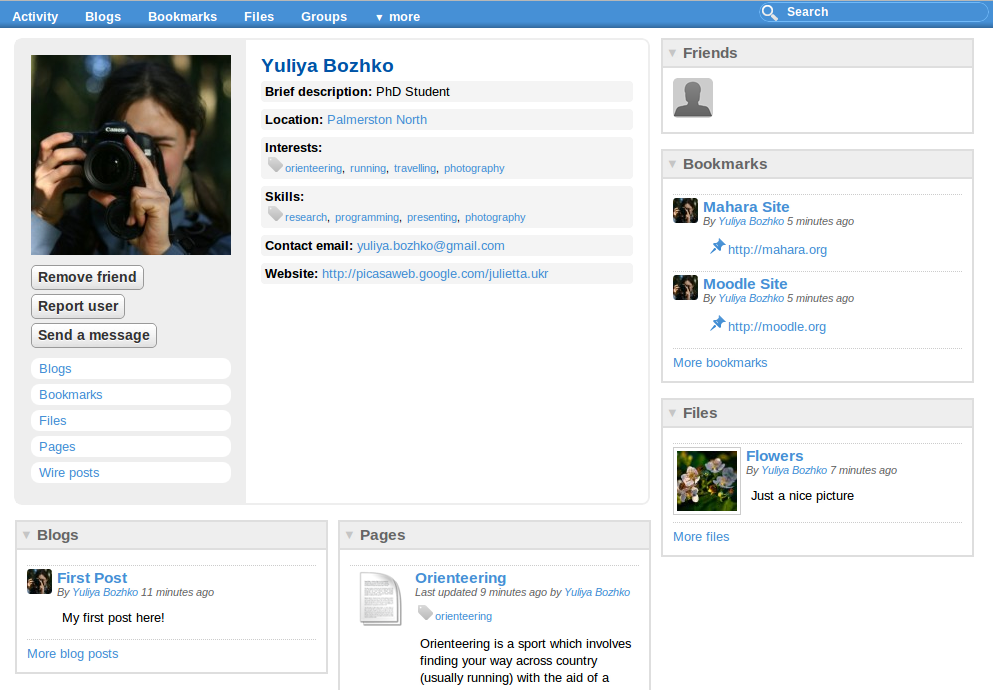
\includegraphics[width=0.9\textwidth]{CH4-F5-ELGG}}
\caption{ELGG 1.8 example}
\label{fig:elgg}
\end{figure}

Similarly to some other \ep~systems, ELGG has groups for collaboration. Groups
have the same system components (e.g. blogs, pages, files) as single profiles,
and these options can be set up or removed at any time.

ELGG has no reporting system for users which would show a number of page
visits, file downloads, etc. However, minor reporting functionality is available
for administrative purposes.

In 2007, interoperability between ELGG and the open source LMS Moodle was
established for single sign-on and courses integration. However, since Moodle
1.9 there is no news on plugin updates. Information has been found on the
Internet about a proprietary plugin being developed for ELGG-Moodle integration,
although no up-to-date documentation is currently available that would describe
this plugin.
 
\subsubsection{Mahara}
Mahara\footnote{\url{http://mahara.org} (Accessed April 16, 2012)} is an open
source \ep~system started by a group of education academics at Massey University in 2006 funded by the New
Zealand Tertiary Education Commission \citep{Brown2007}. The system is a
standalone application and does not require any kind of LMS or other system
installed. Its modular and extensible architecture resembles the architecture of
Moodle LMS. This can be explained by the fact that developer community of Mahara
is deeply involved in the Moodle community. The system is claimed to be highly
\textit{pluggable} which allows adding various Web 2.0 web services and
establish interoperability with other systems \citep{MaharaGovernanceGroup2011}.

Mahara functionality includes a number of standard \ep~features like file
repository, reflection tools in form of blogs, presentation and sharing tools as
well as elements of social networking like friends lists, forums, message board
and e-mail. Mahara has an internal r\'{e}sum\'{e} builder which allows users to
create their digital CV with various information options. Sharing is done
through pages which are called \textit{views} (Figure \ref{fig:maharaep}). Users can
create single views or collections of views and fill them with artifacts from
their \ep~repository. Views can be created from scratch as well as from a
template developed by another user.

\begin{figure}[htb]
\centering
\setlength\fboxsep{0pt}
\setlength\fboxrule{0.5pt}
\fbox{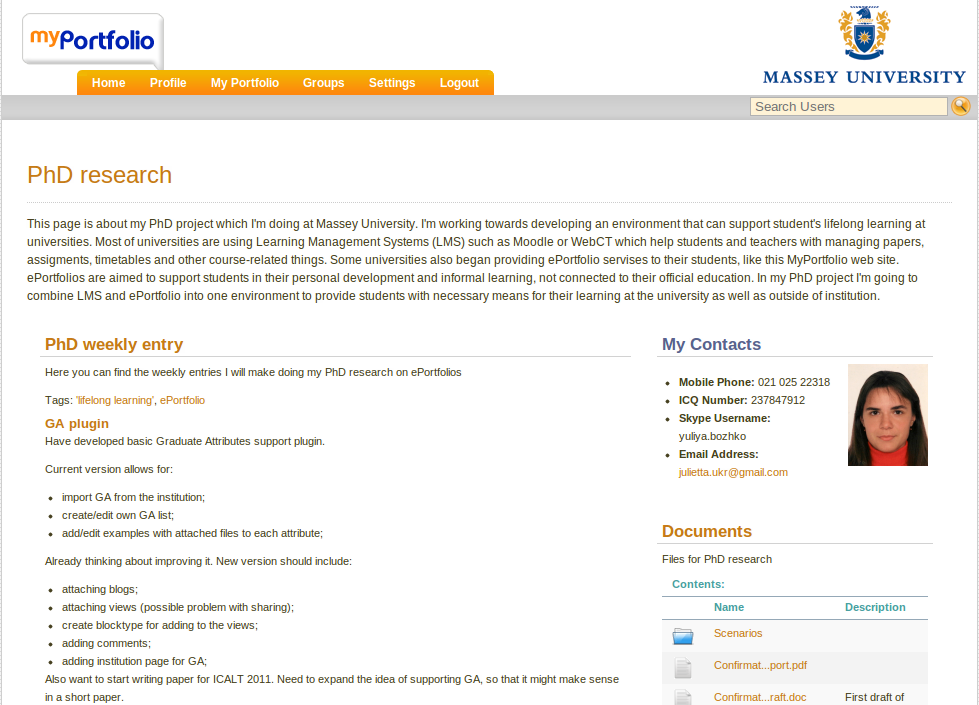
\includegraphics[width=0.95\textwidth]{CH4-F4-Mahara}}
\caption{Mahara ePortfolio 1.3 example}
\label{fig:maharaep}
\end{figure}

A group portfolio is available for collaboration purposes. Compared to personal
accounts, groups have functionality limited to creating and maintaining pages
(views), forums and file repository.

As it became popular in \ep~systems throughout the recent years
\citep{Waters2009}, Mahara comes with a user-to-user permissions control. Users
can set up three levels of access to parts of their \ep s (private, individual
and public) which defines what items and information others can see. Currently
the Mahara system does allow sharing views with others or making them public,
but giving feedback is restricted to registered users.

Mahara supports a complete LEAP2A interoperability
\citep{MaharaGovernanceGroup2011} which allows the import of portfolio content
to Mahara and export to another \ep~system, provided that this interoperability
standard is implemented on the other side. In addition, export in form of static
HTML pages is supported.

The latest version of Mahara supports single sign-on with Moodle, which means
that users can log on to both systems using only one account. Unofficial plugins
developed by the community allow for submitting views as assignments to Moodle.
However, this functionality is not included in official release. The road-map of
Moodle 2.0 included a repository plugin for Mahara that would allow direct
export of artifacts from LMS to \ep. Meanwhile, Moodle 2.1.1 release still does
not support this functionality.

\subsubsection{PebblePad}

PebblePad\footnote{\url{http://www.pebblepad.co.uk}} is a proprietary web-based
\ep~system. However, its designers tend to call it not just an \ep~system, but
Personal Learning System that can be used in a variety of learning contexts
\citep{PebbleLearningLtd2010}. The system is popular and primarily used in the
UK Higher Education sector and has been involved in a number of JISC funded
ePortfolio research projects including such projects as 
ePistle\footnote{\url{http://jisc.ac.uk/whatwedo/programmes/edistributed/epistle}
(Accessed April 16, 2012)} and
File-Pass\footnote{\url{http://jisc.ac.uk/whatwedo/programmes/edistributed/filepass} (Accessed April 16, 2012)}.

According to the PebblePad technical specification, the back-end of the system
requires Windows and SQL Servers to run. The front-end uses Flash, which can
create a challenge for the web application's accessibility, usability and
performance. To function, Flash-based applications require a plugin which in
turn might cause many standard browser features not to perform as the user would
expect or may even cause a browser crash. Flash applications do not work on many
mobile and portable devices. In addition, because Flash applications are
compiled into binary files, screen readers used on web sites that support the
sight impaired cannot read them which results in poor accessibility.

PebblePad has a customizable user interface (Figure \ref{fig:ppep}) which
includes user-defined size and style of text and background colours.
Institutions can have their own interface that fits in with the institutional
branding.

\begin{figure}[htb]
\centering
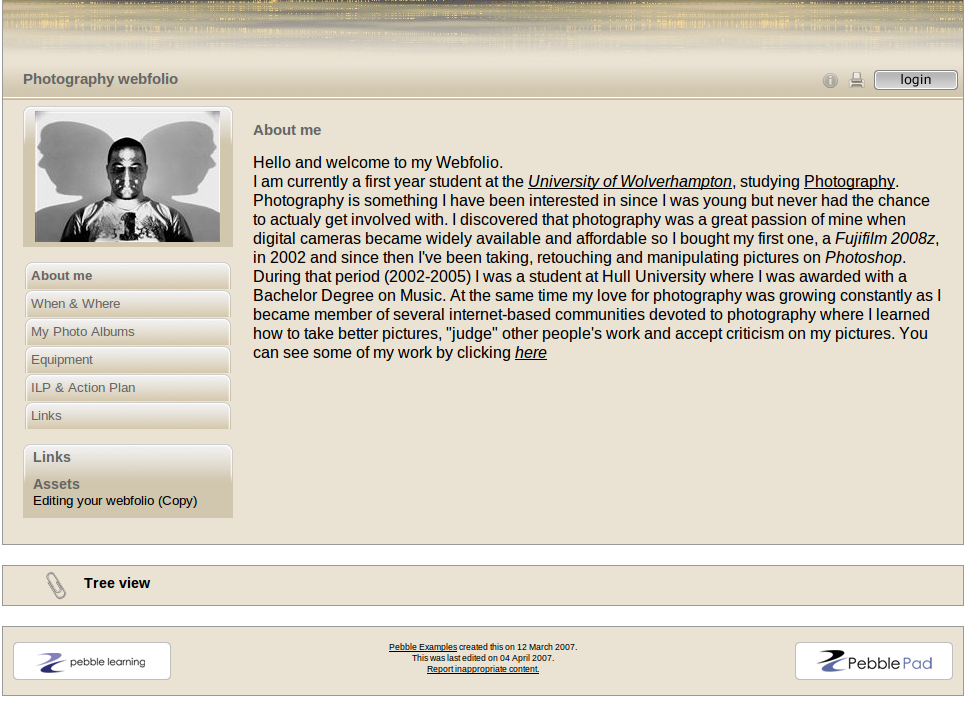
\includegraphics[width=0.9\textwidth]{CH4-F3-PebblePad}
\caption[PebblePad \ep~system example]{PebblePad \ep~system example
\citep{PebbleLearningLtd}}
\label{fig:ppep}
\end{figure}

Items stored in the PebblePad repository are called assets. There are thirteen
asset types that are subdivided into three core types, namely: uploaded files,
single assets and aggregating assets. Creation of some assets can be guided by
step-by-step wizard. Assets can be shared with others, inside or outside of an
institution, for a certain period of time through user-defined permissions. If a
person, who needs to see an asset, is not a part of the PebblePad community, a
temporary username and password will be automatically created allowing them to
view a shared asset. Assets allow for setting up a wide range of permissions,
which can include commenting and copying rights, collaboration and re-sharing
of a shared asset with a third party.

However, despite these features, working with assets in PebblePad has its
disadvantages. The way the system's repository is structured, asset tracking and
finding in PebblePad is noted to be not user-friendly \citep{Overton2009}. Due
to poor asset management, users can end up deleting files and breaking links
between assets, or forgetting to update the hyperlinks of the changed assets,
which results in missing files for someone who is viewing the asset. Users
cannot upload files larger than 10MB.

PebblePad has an interface with the Moodle LMS that allows \ep~users to have
single sign-on with LMS and also export items from Moodle to their ePortfolio.
The system supports Leap2a and IMS eP as well as import from any RSS or Atom
compliant system. According to the vendor's website, as at the middle of 2011,
the price of PebblePad adoption ranged from 14,95GBP per year for individual
accounts hosted by the company to 1GBP per user per year for the largest
customers hosting the system themselves. After graduation from the sponsoring
institution, students can get a free 12-month personal account managed by Pebble
Learning.

\subsubsection{Discussion}
The overview of the \ep~systems showed that they have relatively standard set of
features. All systems provide support for the key \ep~processes of collecting,
selecting, reflecting, planning and connecting as described in Section
\ref{sec:charep}. Collecting is usually done through gathering various files and
creating records in the systems. After information capturing is finished, user
can sort artifacts selecting the ones that can be used for intended purpose.
Reflection in the majority of the \ep~systems is supported through personal
blogs. Some systems (eFolio, PebblePad) also provide reflection options linked
directly to the individual artifacts. Planning is implemented in the form of
personal learning objectives or learning plans, although not all \ep~systems
have this feature. Connecting of artifacts is largely achieved through web pages
or other internal aggregation methods. All reviewed \ep~systems allow meaningful
collections of artifacts to be shared for feedback and assessment purposes.

Apart from common functionality, some of the \ep~systems have unique features
not present in the majority of other systems. Among these are:
\begin{itemize}
  \item Creating audio recordings within the \ep~environment (Desire2Learn)
  \item Individual items can have multiple reflections (eFolio)
  \item Social networking features (e.g., friends lists, message board, etc.)
  (ELGG, Mahara)
  \item Threaded topics for reflection (BlackBoard \ep)
  \item Initial set-up wizard (BlackBoard \ep, eFolio)
  \item Pluggable interface (ELGG, Mahara)
  \item Sharing of individual artifacts (eFolio, PebblePad)
\end{itemize}

\begin{sidewaystable} \scriptsize
\centering
	\caption{Mapping \ep~systems' features against \LLLs guidelines}
	\begin{tabular}{|c|p{3.25cm}|p{3.25cm}|p{3.25cm}|p{3.25cm}|p{3.25cm}|p{3.25cm}|}
	\hline
	 \multicolumn{1}{|c|}{} &
     \multicolumn{1}{c|}{\textbf{BlackBoard ePortfolio}} & 
     \multicolumn{1}{c|}{\textbf{Desire2Learn}} & 
     \multicolumn{1}{c|}{\textbf{eFolio}} & 
     \multicolumn{1}{c|}{\textbf{ELGG}} & 
     \multicolumn{1}{c|}{\textbf{Mahara}} & 
     \multicolumn{1}{c|}{\textbf{PebblePad}} \\ \hline
	\textbf{G1} & 
	Combination of \ep~and LMS supports all types of learning & 
	Combination of \ep~and LMS supports all types of learning & 
	Potential integration with Moodle LMS can cover support for all types of
	learning \textit{(No reliable information found)} & Potential single sign-on
	with Moodle LMS can cover support for all types of learning \textit{(No
	reliable information found)} & Integration with Moodle LMS covers support for
	all types of learning & Integration with Moodle LMS covers support for all
	types of learning \\ \hline \textbf{G2} & 
	-- Initial guidance through \ep~set-up wizard; \newline -- Guidance through
	 course goals and objectives; \newline -- Feedback in form of comments on
	web pages & -- Feedback on various types of artifacts; \newline -- Guidance
	through predefine competences in LMS; \newline -- Templates can be used as
	guidance & -- Feedback on various types of artifacts; \newline -- ``Getting
	started" Wizard for initial set-up & 
	Feedback on web pages and individual artifacts & 
	Feedback on web pages and artifacts on web pages; \newline -- Templates of web
	pages can be used as guidance & 
	Feedback on assets can be provided as guidance for students \\ \hline 
	\textbf{G3} & 
	-- Lecturers can define learning objectives; \newline -- Lecturers can provide
	feedback on shared resources & 
	-- Lecturers can define competences in LMS; \newline -- Lecturers can
	provide feedback and evaluate; \newline -- Lecturers can create templates for
	evaluations & 
	-- Lecturers can provide feedback on shared resources; \newline -- Lecturers
	can create templates to map competencies & 
	-- Lecturers can set up questionnaires; \newline -- Lecturers can provide
	feedback & 
	-- Lecturers can provide feedback on shared resources; \newline -- Lecturer
	can create templates of web pages & 
	Lecturers can provide feedback on shared assets	\\	\hline 
	\textbf{G4} & \textit{No information found} & \textit{No information found} &
	\textit{No information found} & \textit{No information found} & 
	\textit{No information found} & \textit{No information found} \\ \hline 
	\textbf{G5} & 
	\textit{No information found on collaboration} \newline -- Communication is
	in form of comments or through message center & 
	-- Collaboration through sharing; \newline -- Enhanced communication through
	LMS features & 
	\textit {No support for collaborative activities} \newline Integrated
	communication tools & 
	-- Groups are used for collaboration; \newline --	Communication is in 
	the form of comments, message board and internal message system & 
	-- Groups are used for collaboration; \newline -- Communication is
	in the form of comments, wall messages and internal message system & 
	-- Collaborative work with assets; \newline -- Communication is
	in the form of comments; \newline -- Assets re-sharing \\
	\hline 
	\textbf{G6} & 
	Data and grades export from LMS to \ep & 
	Data and grades export from LMS to \ep & 
	\textit{No information found} & 
	\textit{No data integration with external sources or LMS} & 
	Data export from LMS to \ep & 
	Data export from LMS to \ep \\ \hline
	\textbf{G7} & 
	-- Users can define learning objectives; \newline -- Users can
	associate artifacts with learning objectives & 
	-- Achievements can be recorded in form of presentations; \newline -- Users can
	set up personalized learning plans & 
	Mapping of specific competencies and learning outcomes into individual
	portfolios & 
	No specialized way or recording achievements. Blogs and pages can be used for
	this purpose & 
	-- Achievements are described as a part of user profile; \newline -- Users can
	create goals in form of plans & 
	Achievements can be recorded through the assets ``achievements''
	and ``experiences''	\\ \hline 
	\textbf{G8} & 
	Addressing high-order skills through defined by lecturers learning
	objectives / course goals & 
	Addressing high-order skills through assessment rubrics or integration with LMS
	& 
	Addressing high-order skills is done in form of web pages or tied to
	institutional rubrics & 
	Addressing high-order skills is done in form of web pages & 
	Addressing high-order skills is done in form of web pages & 
	Addressing high-order skills can be done in form of web pages or assets \\
	\hline 
	\textbf{G9} & 
	Reflections are in form of blogs and threaded topics & 
	-- Forms can be used for self-evaluation; \newline -- Reflections are a
	separate form of artifacts & 
	Individual items can have multiple reflections & 
	Reflection in the form of blogs & 
	Reflection in the form of blogs & 
	-- Reflection through wizard when creating assets; \newline -- Reflection in
	the form of blogs \\ \hline
	\end{tabular}
\label{tab:ep2map} 
\end{sidewaystable} 

Reviewing the \ep~systems from the \LLLs perspective requires looking further
than the key \ep~processes and activities. Suitability and ability of the
systems to provide support for \LLLs should be evaluated against the guidelines
and recommendations discovered in the literature (Section \ref{sec:needs}). Table
\ref{tab:ep2map} shows possible mapping of these recommendations to the features
of the reviewed \ep~systems. 

Exploration of these features from the \LLLs perspective showed that not all
guidelines are followed or supported by the \ep~systems. Particularly, no
information was found on the \ep~systems helping students to understand how they
learn and develop their skills through better organized learning materials.
However, while rigorous analysis has been attempted, a number of reasons have
hindered this analysis and suggest caution when looking at the findings.
Firstly, in some cases no reliable information was found to make unambiguous
conclusion. Secondly, the majority of proprietary systems were reviewed relying
on the sources of information other than first-hand experience of the researcher
which might have influence their trustworthiness. Finally, the guidelines
provided in the literature were not formal requirements and therefore their
assessment was largely done using analogical reasoning. Due to these issues, a
further exploration of the \ep~systems from the \LLLs perspective is required,
and the next section provides additional reasons for this.

\subsection{\ep~Systems in Light of Lifelong Learning}

Considering that the expectation around \ep~systems is that these systems
support \LLLsn, the question is whether they are doing it effectively in light
of the recommendations identified in the literature. Due to the fact that the
literature provides only highly conceptual recommendations, it is difficult to
translate these into formal requirements. Therefore, assessment whether these
recommendations are met by the features implemented in the systems turns into a
challenging task. 

The previous section described an attempt to address this problem trying to map
the recommendations against the features of the reviewed \ep~systems. However,
due to the highly conceptual level of these recommendations, the results of this
analysis should not be considered complete and final. As was explained earlier,
common sense and personal experience had to be followed to perform this
analytical mapping. To solve this problem, bringing the recommendations to the
practical level is the next important step towards a better understanding of
what is expected from the environment that can support \LLLsn. One can argue
that the majority of these recommendations cannot be addressed by just providing
an improved system \citep{Schaffert2008}. However, from another perspective, a
better system might aid to supporting various important aspects of learning that
usually stay outside of focus of many learning environments.

Although no prior research was found that would look at the \ep~systems from the
\LLLs perspective, there are a number of issues known among the \ep~community
that might be relevant to \LLLs support. For example, current \ep~systems have
difficulty helping students to link abstract knowledge to practical experience
which is an important part of understanding one's personal progress and
achievements \citep{Chou2009}. Interoperability between different \ep~systems as
well as other learning systems is quite poor despite the existing standards
\citep{Clark2011}. Assuming that \ep s are lifelong, they are supposed to cope
with large amounts of data \citep{Butler2010}. However, practice shows that
current systems can barely offer efficient methods for managing data
repositories to users who have been using them extensively for just a couple of
years. There are also issues of ethics, privacy and intellectual property where
\ep~users need to decide who owns the data and how it can be used
\citep{Challis2005}.

The problems mentioned here are just some examples that are not likely to draw a
complete picture. To get a deeper insight into \ep~issues and understand what
improvements are required for \ep~systems to fulfil the promise of efficient
\LLLs support, a deeper analysis of the area is required.

\section{Summary}

Based on the deliberations outlined in this chapter, additional conceptual
requirements can be considered along with the recommendations for successful
\LLLs support, such as:

\begin{itemize}
	\item A good virtual learning environment should facilitate the development of
	\LLLs skills;
	\item It should fit the university needs;
	\item It should fit the learners' needs and be accepted by students. 
	\item It should create a bridge between institutional and personal learning.
\end{itemize}

\ep~system seems to fit well into this picture. It brings a balance into the
world of learning environments, and has potential of closing the gap that exists
between LMS and Web 2.0. As was discussed earlier, LMS cannot provide the
required level of support for \LLLs as it is focused primarily at supporting
formal education. While Web 2.0 tools have the potential to do so, providing
quality of service for these tools in institutional settings is not feasible.

Reviewing \ep~systems showed that the systems currently available world-wide
offer a range of opportunities for \LLLsn. Each system comes with commonly
valuable functionality that promises support for important aspects of learning.
However, are they mature enough to be a part of the environment that provides
comprehensive support for \LLLsn? The previous section discussed that current
\ep~systems might still lack some elements important for \LLLsn. To support this
hypothesis, the next chapter will explore the needs for \LLLs supported by
\ep~systems based on the major stakeholders perspective. University students and
lecturers have been interviewed to get their insight on the requirements and to
understand whether these comply with the literature review findings.
